\section{SYSTEM DESIGN AND ARCHITECTURE}
\vspace{1mm}
\subsection{System Overview}
\begin{figure}[h]
    \centering
    \vspace{2mm}
    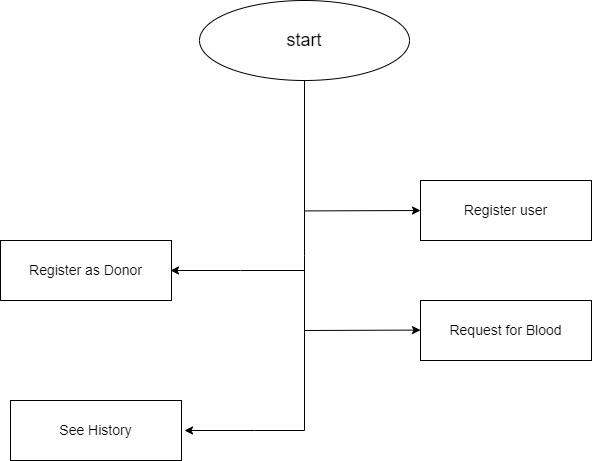
\includegraphics[width=120mm]{images/systemoverview.jpg}
    \caption{System Overview}
    \label{fig:System overview}
\end{figure}
\newpage
\subsection{Use Case Diagram}
\begin{figure}[h]
    \centering
    \vspace{4mm}
    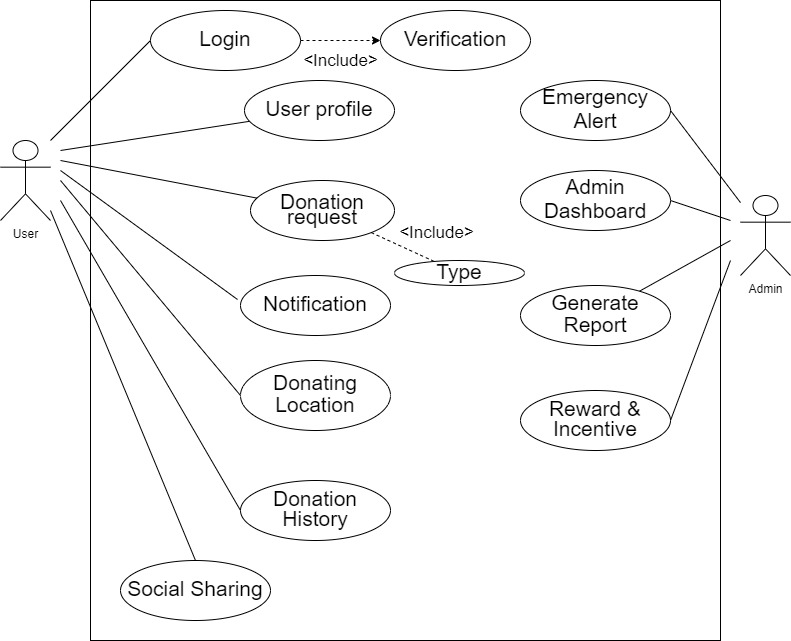
\includegraphics[width=140mm,height= 170mm]{images/UsecaseFinal.jpg}
    \caption{Use Case Diagram}
    \label{fig:Use Case Diagram}
\end{figure}
 \newpage
\subsection{Data Flow Diagram}
\begin{figure}[h]
    \centering
    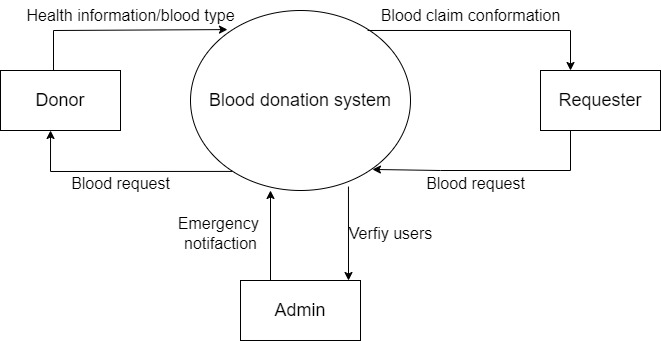
\includegraphics[width=140mm, height= 50mm]{images/DFD0.jpg}
    \vspace{2mm}
    \caption{Level 0 DFD Diagram}
    \label{fig:level 0 DFD}
\end{figure}
\vspace{0.5in}
\begin{figure}[h]
    \centering
    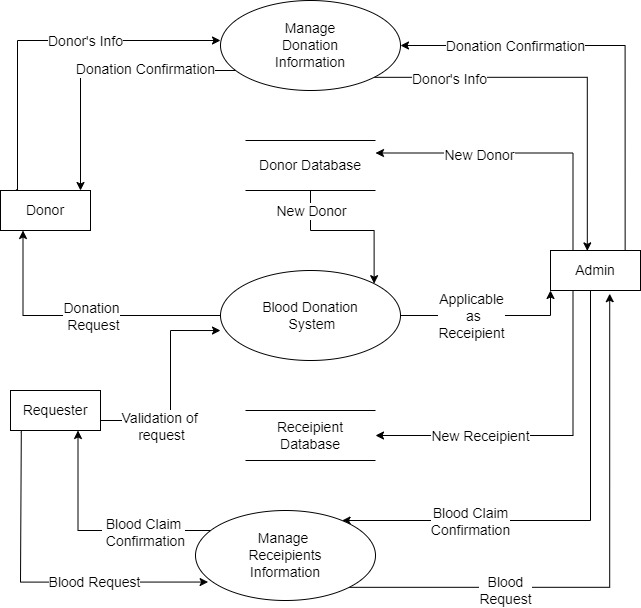
\includegraphics[width=140mm, height = 100mm]{images/dfd1.jpg}
    \caption{Level 1 DFD Diagram}
    \label{fig:level 1 DFD}
\end{figure}

\newpage
\subsection{Activity Diagram}
\begin{figure}[hbt!]
    \centering
    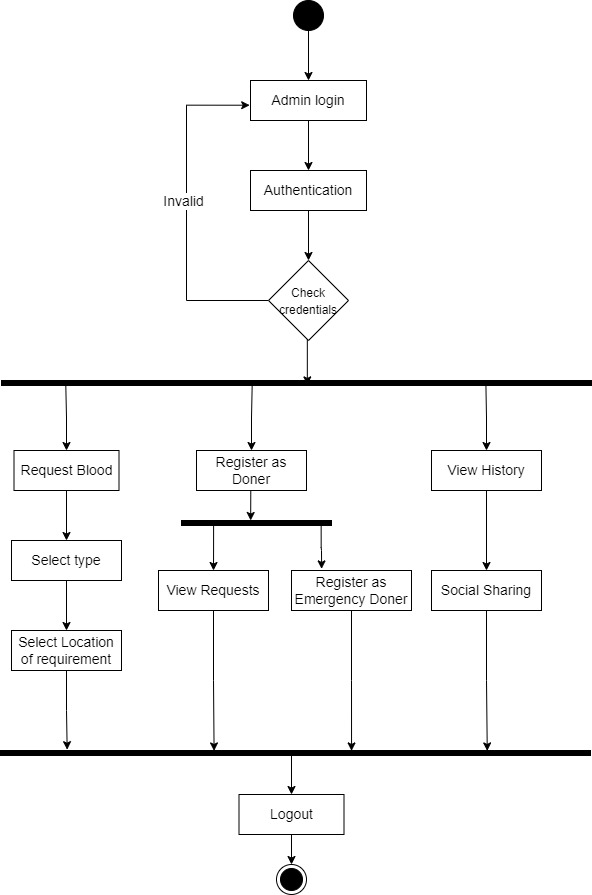
\includegraphics[width=145mm]{images/activity.jpg}
    \caption{Activity Diagram}
    \label{fig:Activity Diagram }
\end{figure}

\newpage
\subsection{Sequence Diagram}
\begin{figure}[hbt!]
    \centering
     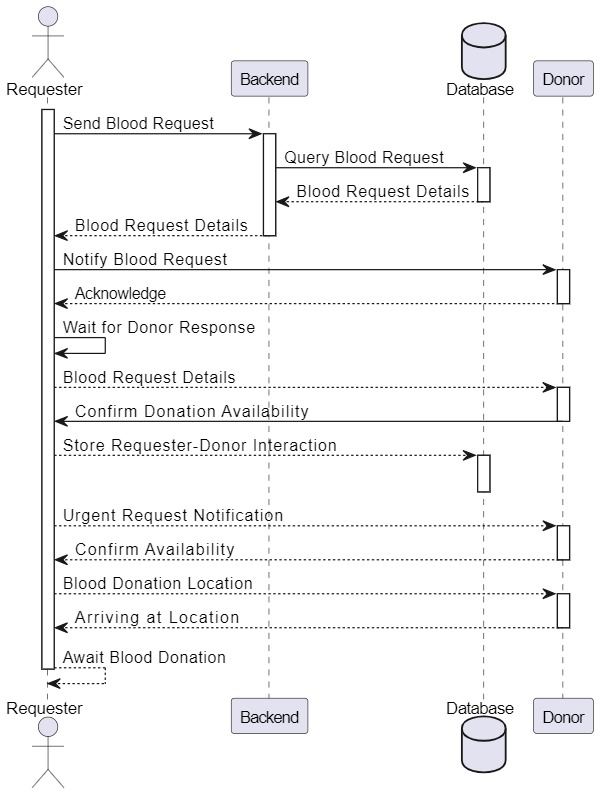
\includegraphics[width=145mm]{images/sequential.jpg}
    \caption{Sequence Diagram For Requesting And Accepting Blood Request}
    \label{fig:Sequence Diagram}
\end{figure}
%\newpage
%\subsection{Class Diagram}
%/\begin{figure}[hbt!]
%    \centering
 %    \includegraphics[width=150mm]{class.jpg}
  %  \caption{Class Diagram for \textit{Life Tracker} web-app }
   % \label{fig:Class Diagram}
%\end{figure}
